\section{Detektion von Snooker-Kugeln}\label{kap:snooker_detection}

Ziel ist es, die Position, d.h. den Kugelmittelpunkt, jeder Kugel in Pixelkoordinaten so genau wie möglich zu bestimmen.
Diese Pixelkoordinaten können anschliessend wie in Kapitel \ref{kap:model_coordinate_system} beschrieben in ein
Modellkoordinatensystem umgewandelt werden, welches für die weitere Verarbeitung genutzt werden kann.

Die Anwendung des Circle Hough transform \cite{circle_hough} für die Extraktion der Kugeln ist naheliegend, führt allerdings auf dem
Graustufenbild dazu, dass auch Schatten als Kugeln detektiert werden. Diese gilt es zu vermeiden,
weshalb zunächst eine Segmentation aufgrund anderer Eigenschaften erfolgen muss.
In Abbildung \ref{fig:input_with_shadows} ist das Eingabebild mit Schatten abgebildet.

\begin{figure}[h!]
    \begin{center}
    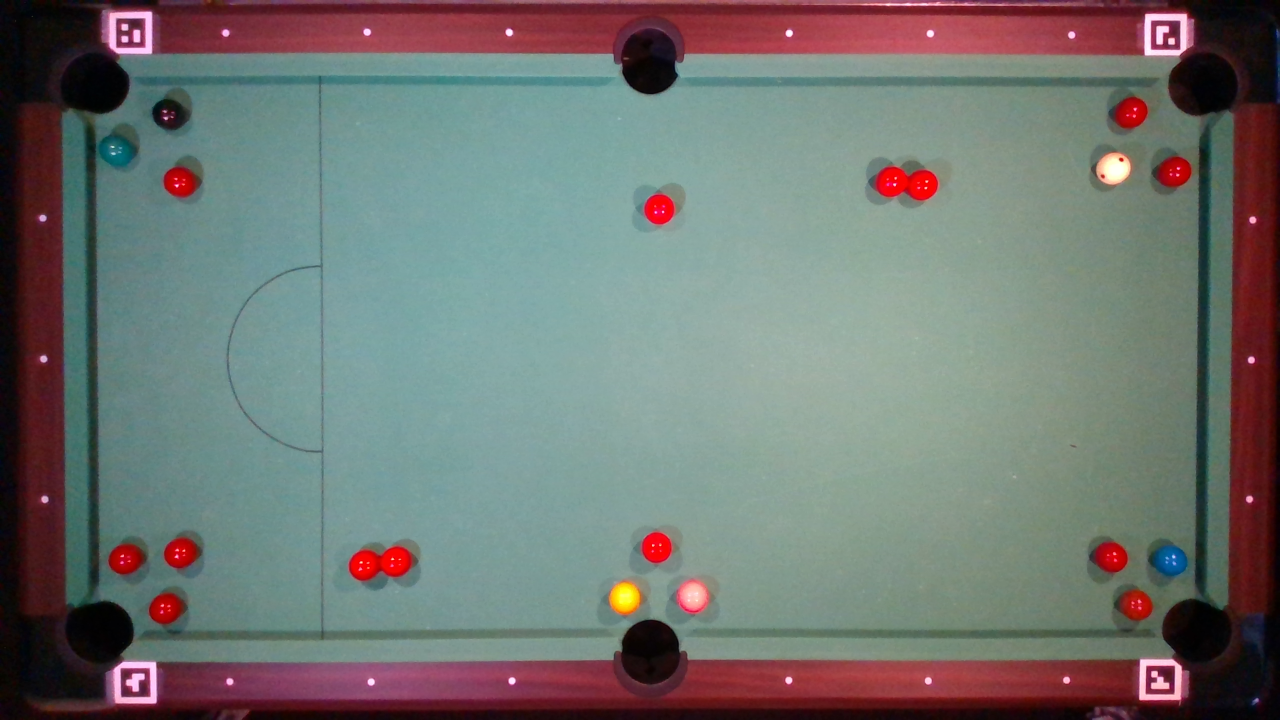
\includegraphics[width=0.8\linewidth]{../common/resources/detection/input.png}
    \end{center}
    \caption{Eingabebild mit Schatten}
    \label{fig:input_with_shadows}
\end{figure}

Zunächst wird ein Gaussfilter mit der Kernelgrösse von 5x5 auf das Eingabebild angewendet, um Rauschen zu unterdrücken.
Anschliessend wird das Bild vom RGB-Farbraum in den HSV-Farbraum \cite{hsv_color_space} umgewandelt, um eine einfacher
Segmentation zu ermöglichen, weil dadurch einzelne Eigenschaften wie Farbwert, Sättigung und Helligkeit gefiltert werden können.

Des weiteren sollen Kreise, welche ausserhalb des Spielfeld liegen, ausgeschlossen werden können.
Dazu wird eine binäre Maske, ein einkanaliges Bild mit den Werten 255 (= wahr) und 0 (= falsch), erzeugt.
In der Maske hat jedes Pixel, an dem ein Kugelmittelpunkt sein darf, den Wert 255, alle anderen den Wert 0.
Das Modellkoordinatensystem wurde in Kapitel \ref{kap:model_coordinate_system} beschrieben.
Die Banden und Löcher des Tisches können in Modellkoordinaten definiert werden, sofern der Tisch ausgemessen wurde.
In Kapitel \ref{kap:model_to_pixel} wurde erarbeitet, wie eine Modellkoordinate in eine Pixelkoordinate überführt werden kann.
Wird diese Transformation für alle Punkte der Banden und Löcher im Modellkoordinatensystem gemacht, können die
entstandenden Pixelpunkte in ein Bild eingezeichnet werden.
Somit kann eine binäre Maske erzeugt werden, welche lediglich das Spielfeld umfasst und damit den Rand des Tisches
und die Löcher aus einem Bild entfernen kann. In Abbildung \ref{fig:table_mask_applied} wurde diese Maske nach Anwendung
auf das Eingabebild aus Abbildung \ref{fig:input_with_shadows} dargestellt.

\begin{figure}[h!]
    \begin{center}
    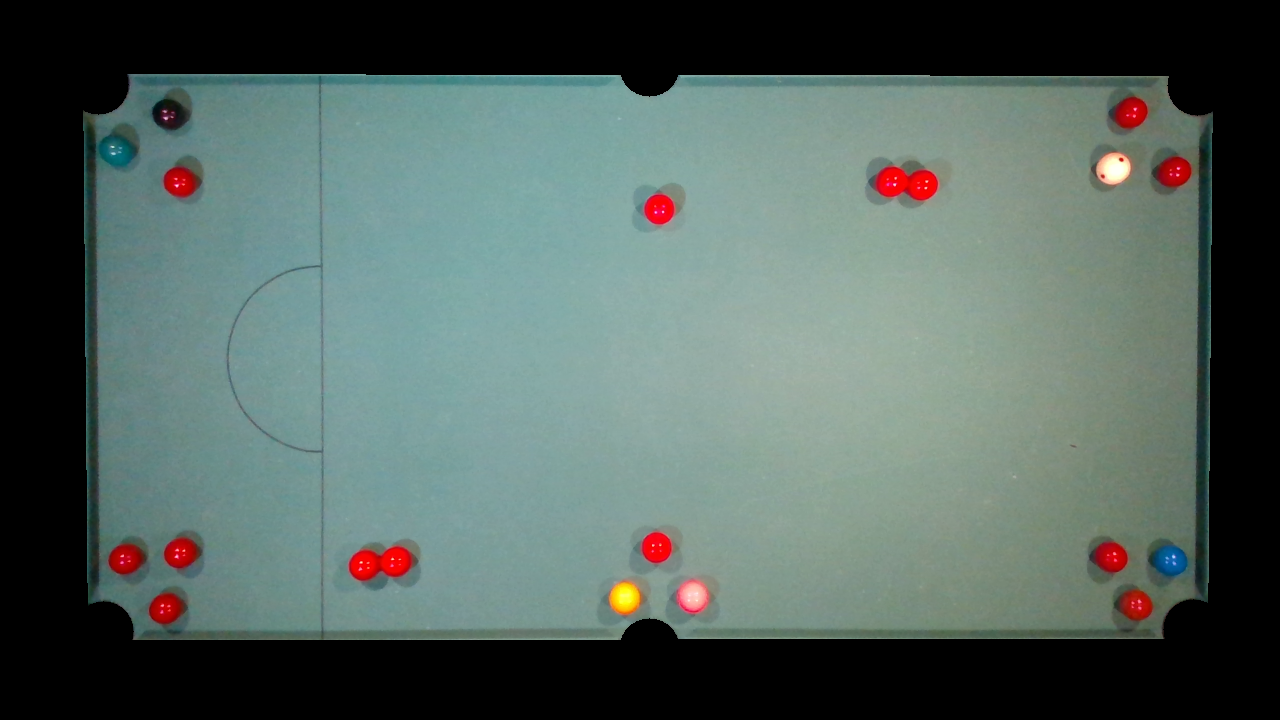
\includegraphics[width=0.8\linewidth]{../common/resources/detection/table_mask_applied.png}
    \end{center}
    \caption{Spielfeld-Maske. Zur Visualisierung auf Abbildung \ref{fig:input_with_shadows} angewendet.}
    \label{fig:table_mask_applied}
\end{figure}

In Snooker gibt es 22 Billiardkugeln, wovon 15 rot, und je eine weiss, schwarz, braun, gelb, grün, blau und pink sind.

Die Erkennung wurde wie folgt aufgeteilt:
\begin{itemize}
  \item Farbige Kugeln (rot, braun, gelb, grün, blau, pink)
  \item Weisse und pinke Kugel
  \item Schwarze Kugel
\end{itemize}

Die Segmentation der farbigen Kugeln erfolgt auf dem Sättigungskanal und diejenige der weissen und schwarzen Kugeln auf dem Helligkeitskanal des Bildes.
Eine Segmentation auf dem Farbwertskanal ist insbesondere für die grüne und blaue Kugel schwierig, weil der Billiardfilz grün ist
und dadurch die Grenze zwischen grünem Tisch und grüner Kugel zu wenig markant ist, siehe Abbildung \ref{fig:hue_green_table_problem}.

\begin{figure}[h!]
    \begin{center}
    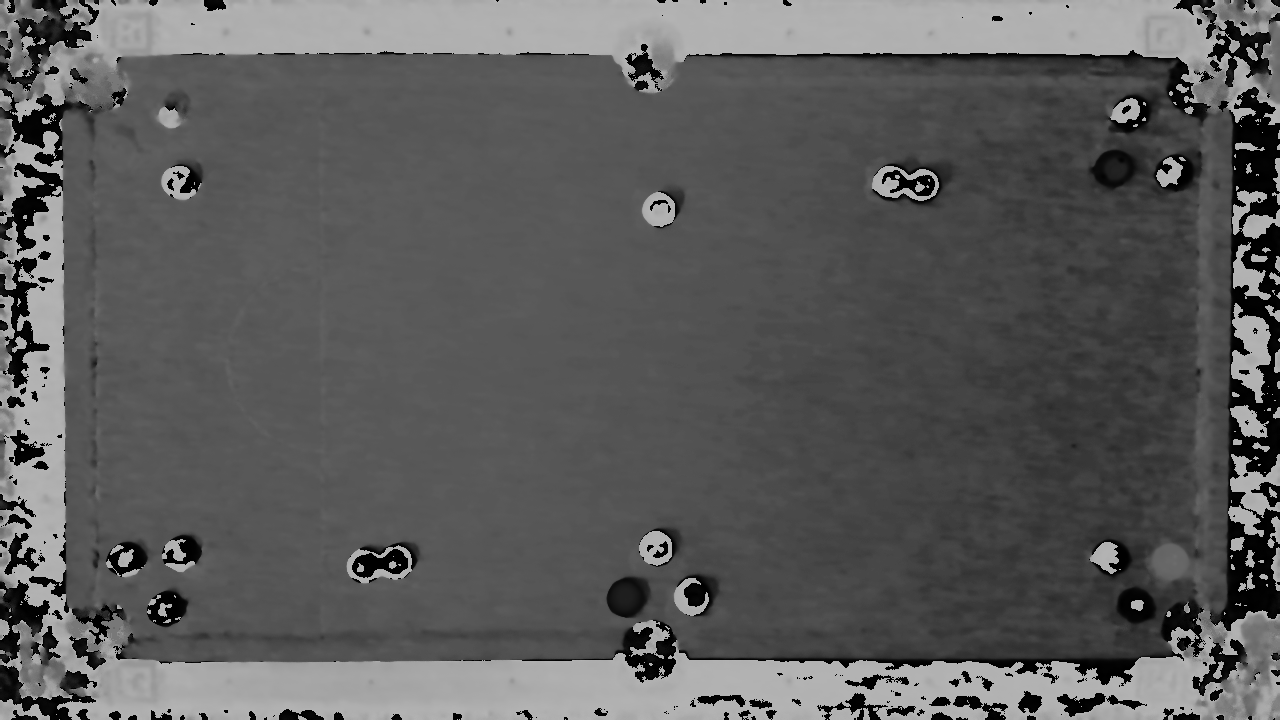
\includegraphics[width=0.8\linewidth]{../common/resources/detection/hue.png}
    \end{center}
    \caption{Der Farbwertskanal. Sehen Sie die grüne Kugel?}
    \label{fig:hue_green_table_problem}
\end{figure}

Die pinke Kugel ist insofern ein Spezialfall, als dass sie je nach Ausleuchtung eine stark gesättigte Farbe oder
eine grosse Helligkeit, ähnlich der weissen Kugel, aufweist. Das bedeutet, dass sie potentiell sowohl aufgrund
der Sättigung als auch der Helligkeit segmentiert wird und dadurch doppelt detektiert wird. Dies gilt es zu verhindern.

Für die Klassifikation der Kugeln, also die Bestimmung der Farbe der Kugel, ist der Farbwert trotzdem sehr sinnvoll.
Die Klassifikation wurde allerdings im Rahmen dieser Arbeit nicht vorgenommen.

Für alle nachfolgend beschriebenen morphologischen Operationen wird ein
rechteckiges structuring element der Grösse 3x3 Pixel verwendet.
Ausserdem ist der gesuchte Kugelradius in Pixel, welcher an den Hough transform übergeben wird, anhand des
Kugelradius in Millimeter berechnet, siehe dazu Kapitel \ref{kap:ballradius_in_pixel}.

Für die farbigen Kugeln mit hoher Sättigung wird ein Filter auf dem Sättigungskanal des HSV-Bilds
angewendet, um eine binäre Maske zu erhalten.

\begin{enumerate}
  \item Aufbau einer binären Maske mittels Filterung auf dem Sättigungskanal des HSV-Bilds.
  \item Morphologisches Opening der binären Maske, um kleine Störpixel zu entfernen.
  \item Morphologisches Closing der binären Maske, um kleine Löcher zu füllen.
  \item Anwendung der binären Maske auf das Graustufenbild, um alle unerwünschten Kugeln auszuschliessen.
  \item Canny edge detection \cite{canny_edge_detection} auf dem maskierten Graustufenbild, um ein Kantenbild zu erhalten.
  \item Hough transform auf dem Kantenbild, um Kreise zu erhalten.
  \item Verwerfen der Kreise mit Mittelpunkten ausserhalb der Spielfeld-Maske.
  \item Verwerfen der Kreise mit Mittelpunkten ausserhalb der binären Maske.
  \item Verwerfen der Kreise mit Mittelpunkten innerhalb der binären Maske der schwarzen Kugel.
\end{enumerate}

Die schwarze Kugel weisst eine geringe Sättigung und kann nicht aufgrund des Farbwerts segmentiert werden.
Das zuverlässigste ist demnach eine Filterung auf dem Helligkeitswert.
Die einzelnen Schritte der Detektion der schwarzen Kugel sind nachfolgend beschrieben:

\begin{enumerate}
  \item Aufbau einer binären Maske mittels Filterung auf dem Helligkeitskanal des HSV-Bilds.
  \item UND-Verknüpfung der binären Maske mit der binären Spielfeld-Maske, um die Löcher und den Rest des Tisches auszuschliessen.
  \item Morphologisches Closing der binären Maske, um kleine Löcher zu füllen.
  \item Morphologisches Opening der binären Maske, um kleine Störpixel zu entfernen.
  \item Anwendung der binären Maske auf das Graustufenbild, um alle unerwünschten Kugeln auszuschliessen.
  \item Canny edge detection auf dem maskierten Graustufenbild, um ein Kantenbild zu erhalten.
  \item Hough transform auf dem Kantenbild, um Kreise zu erhalten.
  \item Verwerfen der Kreise mit Mittelpunkten ausserhalb der Spielfeld-Maske.
  \item Verwerfen der Kreise mit Mittelpunkten ausserhalb der binären Maske.
\end{enumerate}

Die weisse Kugel weisst einen hohe Helligkeitswert auf, welcher zuverlässiger als der Sättigungswert gefiltert werden kann.
Nachfolgend ist der Ablauf der Detektion der weissen Kugel beschrieben.

\begin{enumerate}
  \item Aufbau einer binären Maske mittels Filterung auf dem Helligkeitskanal des HSV-Bilds.
  \item Morphologisches Opening der binären Maske, um kleine Störpixel zu entfernen.
  \item Morphologisches Closing der binären Maske, um kleine Löcher zu füllen.
  \item Anwendung der binären Maske auf das Graustufenbild, um alle unerwünschten Kugeln auszuschliessen.
  \item Morphologisches Closing des maskierten Graustufenbilds, da dadurch die roten Punkte,
  welche auf der weissen Kugel aufgemalt sind, schwächer werden.
  \item Canny edge detection auf dem maskierten Graustufenbild, um ein Kantenbild zu erhalten.
  \item Hough transform auf dem Kantenbild, um Kreise zu erhalten.
  \item Verwerfen der Kreise mit Mittelpunkten ausserhalb der Spielfeld-Maske.
  \item Verwerfen der Kreise mit Mittelpunkten ausserhalb der binären Maske.
  \item Verwerfen der Kreise mit Mittelpunkten innerhalb der binären Maske der farbigen Kugeln, um doppelt detektierte Kugeln, wie etwa die Pinke, zu vermeiden.
\end{enumerate}

Mithilfe der Maske für die weisse Kugel wird teilweise auch die pinke Kugel detektiert,
sofern diese eine geringe Sättigung und hohe Helligkeit aufweist.

Von den übriggebliebenen Kreisen werden die Mittelpunkte extrahiert und dienen als Resultat der Detektion.
Die detektierten Kreisradien sind irrelevant, da der Durchmesser der Kugeln bekannt ist.

Das Resultat der Zusammenführung der detektierten Kreise ist in Abbildung \ref{fig:hough_result} dargestellt.

\begin{figure}[h!]
    \begin{center}
    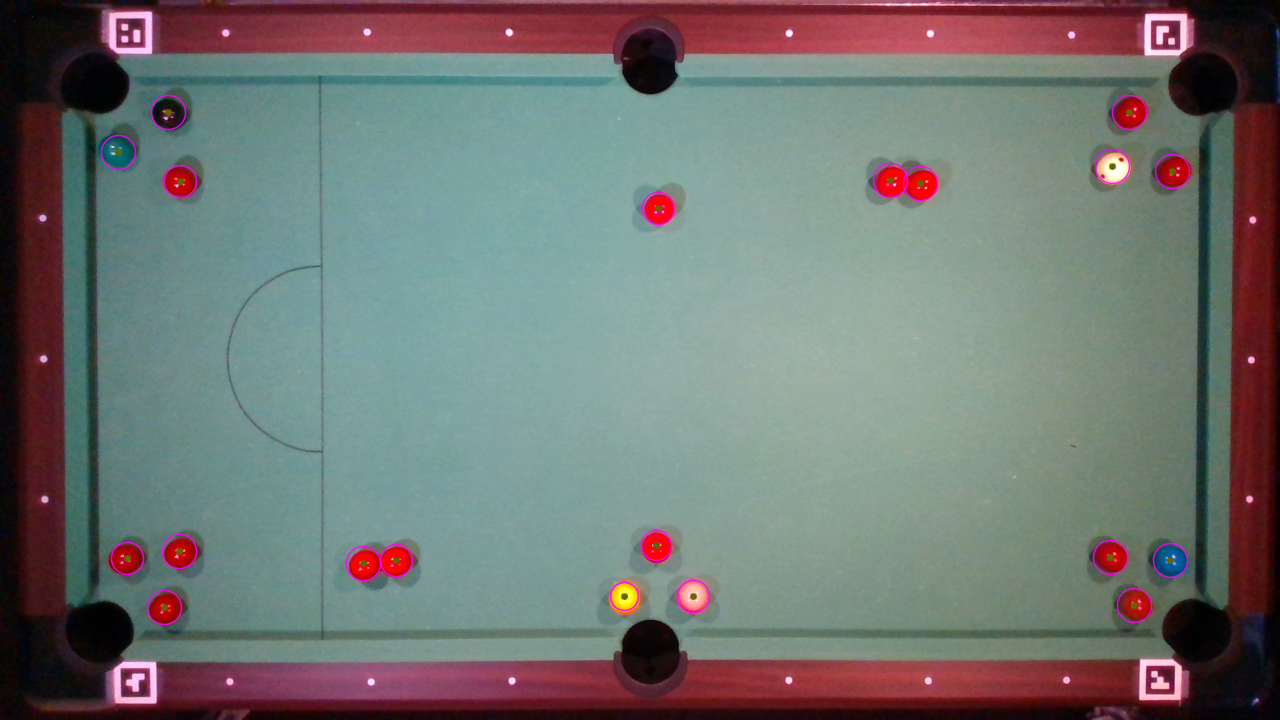
\includegraphics[width=0.8\linewidth]{../common/resources/detection/hough.png}
    \end{center}
    \caption{Resultat der Detektion. Die Kreismittelpunke und -umkreise sind eingezeichnet.}
    \label{fig:hough_result}
\end{figure}
